\documentclass[17pt, a2paper, landscape]{tikzposter}
\usepackage{siunitx}
\usepackage{tabularx}

\title{QEA Boat}
\author{Kawin Nikomborirak, Amy Phung}
\date{\today}

\usetheme{Desert}
\begin{document}
\maketitle

\begin{columns}
  \column{0.4}

  \block{Best Of All Time}
  {
    \begin{tabularx}{0.4\textwidth}{l X}
    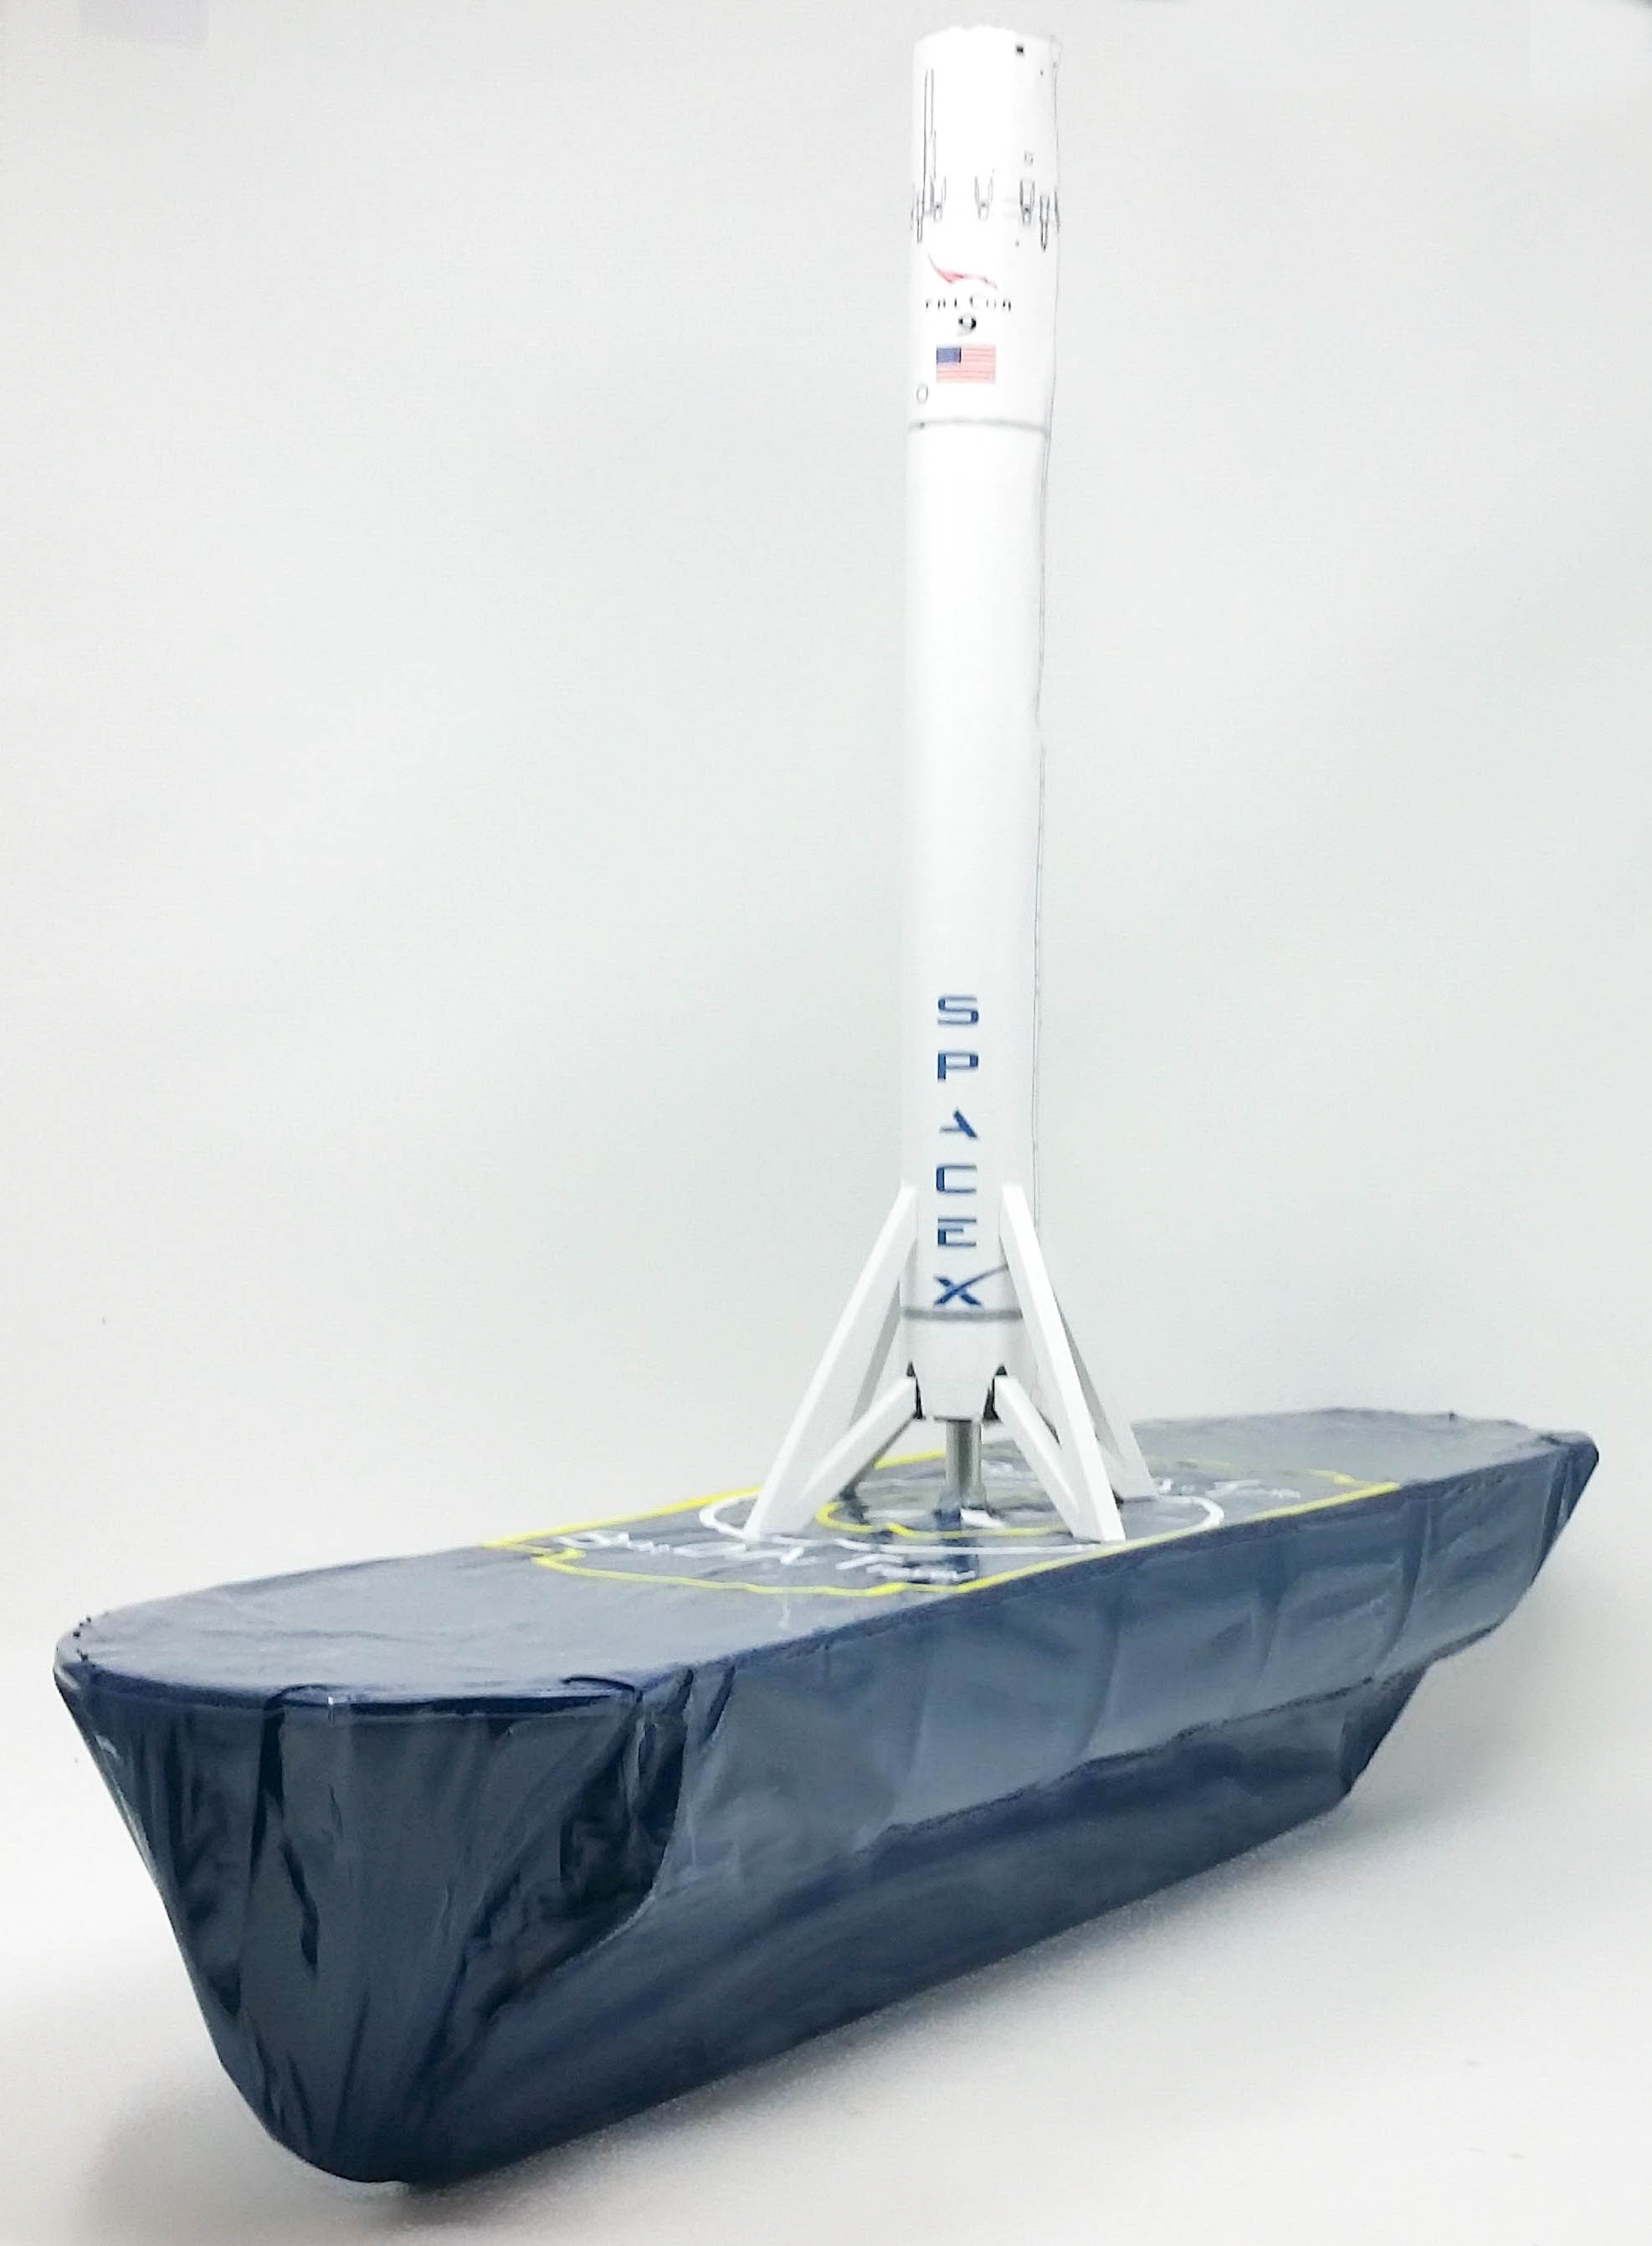
\includegraphics[width=0.18\textwidth]{FinishedBoat.jpg} &
    Boat of Air Transportation
    \end{tabularx}
  }

  \block{Performance Considerations}
  {
    \begin{itemize}
    \item The boat has a functional keel to lower COM.
    \item The AVS should be \ang{130} to best fit between \ang{120} and \ang{140}.
    \item The boat will have little velocity, so minimize the wet surface friction rather than wave breaking friction.
    \item The boat should be as long as possible to eliminate vortices.
    \end{itemize}
  }


  \column{0.6}
  \block{Righting Moment vs Heel Angle}{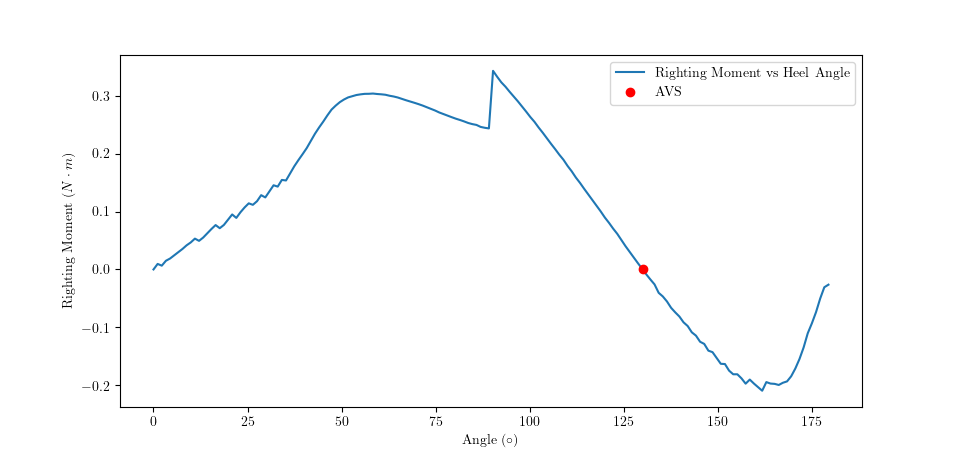
\includegraphics[width=0.53\textwidth]{curve.png}}

  \block{Performance of boats}
  {
    The boat in terms of floating level and AVS was right on the dot.
    The boat cruised at around \SI{.7}{\meter\per\second}, which was slower than other boats and faster than the SolidWorks simulation.
    The speed being faster than SolidWorks is probably due to the nature of fluid simulation, and relative to other boats was three:
    The shrink wrap left a lot of wrinkles which disturbed water flow, as well as having a bit of yaw as it was pulled.
    the surface-area-to-volume ratio of the submerged part, due to concavity, was also suboptimal for slow travel.
  }


\end{columns}

\end{document}
